\documentclass[tikz,border=10pt]{standalone}
\usepackage{tikz}
\usetikzlibrary{positioning, fit, arrows.meta, calc, shapes.geometric}

\begin{document}

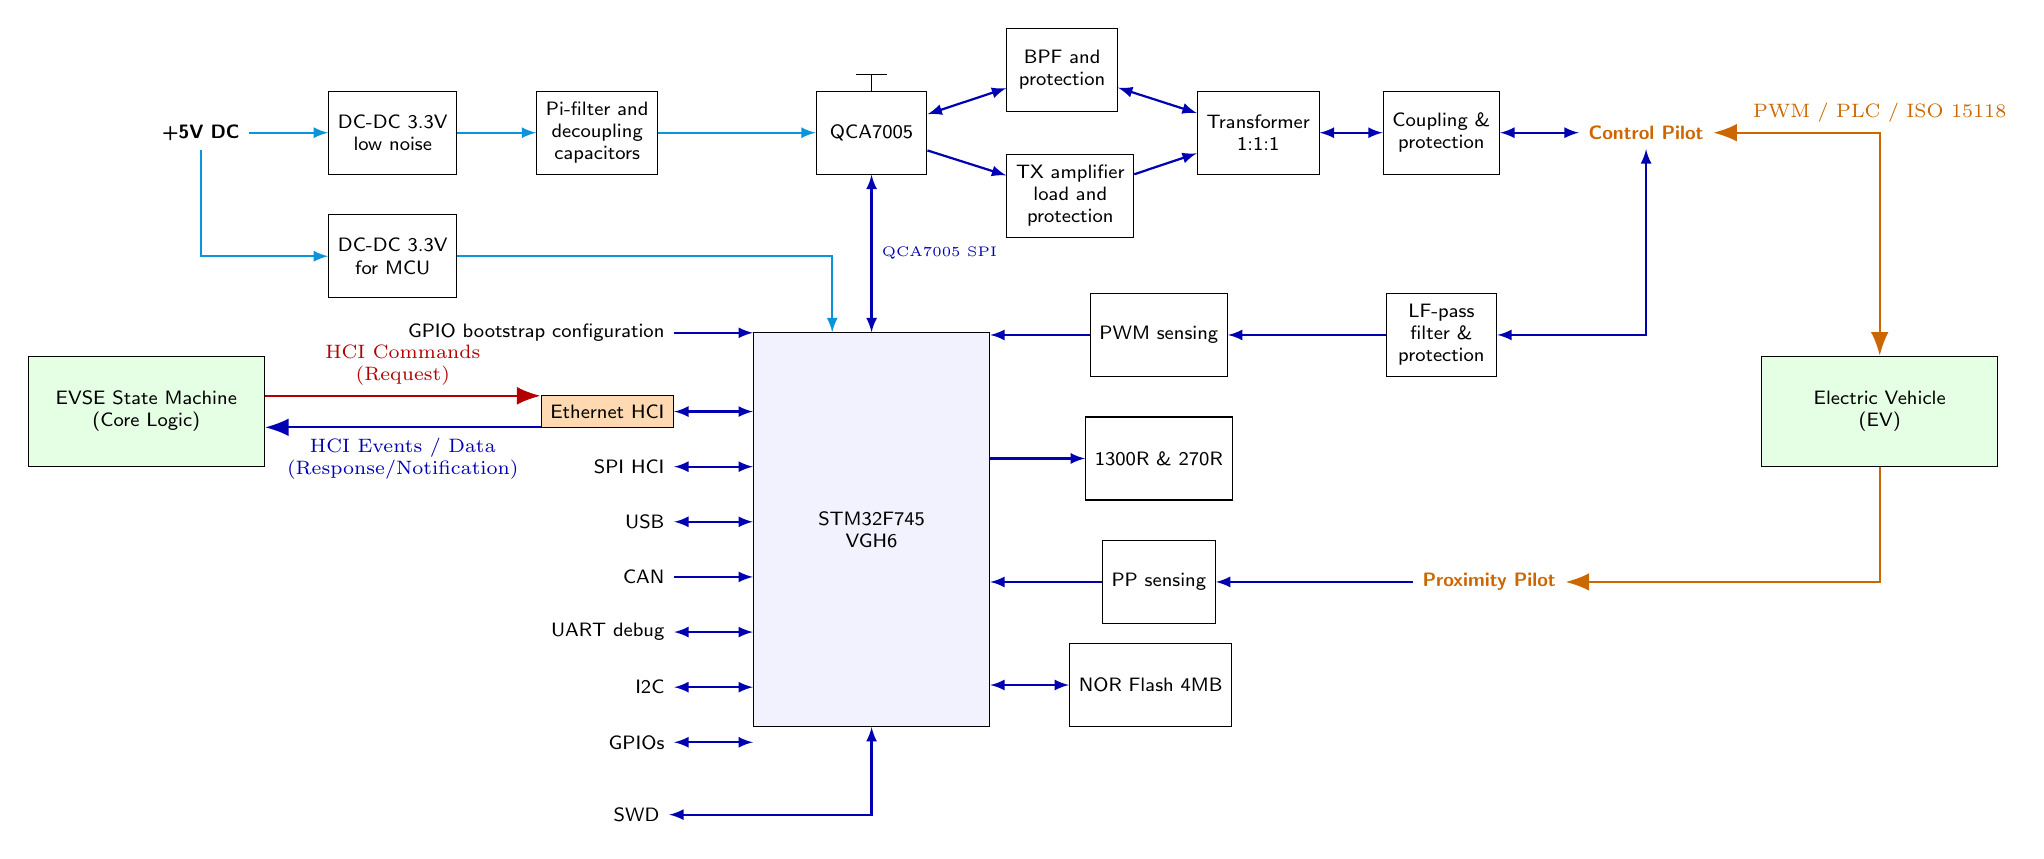
\begin{tikzpicture}[
    node distance=1cm and 1.5cm,
    font=\sffamily\scriptsize,
    block/.style={
        draw, 
        rectangle, 
        minimum height=3em, 
        minimum width=4em, 
        align=center, 
        fill=white
    },
    wideblock/.style={
        block,
        minimum height=4em,
        minimum width=3cm
    },
    line/.style={
        draw, 
        -latex, 
        thick,
        color=blue!70!black
    },
    biLine/.style={
        draw, 
        latex-latex, 
        thick,
        color=blue!70!black
    },
    powerLine/.style={
        draw, 
        -latex, 
        thick,
        color=cyan!80!blue
    }
]

% --- Main Controller (STM32) ---
\node[block, minimum height=5cm, minimum width=3cm, fill=blue!5] (stm32) {STM32F745\\VGH6};

% --- QCA7005 Section (Top) ---
\node[block, above=2cm of stm32] (qca) {QCA7005};

% --- Power Supply Section (Left) ---
\node[block, left=2cm of qca] (pi_filter) {Pi-filter and\\decoupling\\capacitors};
\node[block, left=1cm of pi_filter] (dcdc_qca) {DC-DC 3.3V\\low noise};
\node[left=1cm of dcdc_qca] (v5_in) {\textbf{+5V DC}};

% Move DC-DC for MCU further left to avoid clash with interfaces
\node[block, below=0.5cm of dcdc_qca] (dcdc_mcu) {DC-DC 3.3V\\for MCU};

% --- Interfaces (Left of STM32) ---
\coordinate (stm_left) at (stm32.west);

\node[left=1cm of stm_left, yshift=2.5cm] (gpio_boot) {GPIO bootstrap configuration};
\node[left=1cm of stm_left, yshift=1.5cm, fill=orange!30, draw, rectangle] (eth) {Ethernet HCI};
\node[left=1cm of stm_left, yshift=0.8cm] (spi) {SPI HCI};
\node[left=1cm of stm_left, yshift=0.1cm] (usb) {USB};
\node[left=1cm of stm_left, yshift=-0.6cm] (can) {CAN};
\node[left=1cm of stm_left, yshift=-1.3cm] (uart) {UART debug};
\node[left=1cm of stm_left, yshift=-2.0cm] (i2c) {I2C};
\node[left=1cm of stm_left, yshift=-2.7cm] (gpios) {GPIOs};
\node[above= of stm32, xshift=-0.1cm] (dcdc) {};
\node[below=0.5cm of gpios] (swd) {SWD};

% --- PLC & Analog Front End (Right Top) ---
\node[block, right=1cm of qca, yshift=0.8cm] (bpf) {BPF and\\protection};
\node[block, right=1cm of qca, yshift=-0.8cm] (tx_amp) {TX amplifier\\load and\\protection};

\node[block, right=1cm of bpf, yshift=-0.8cm] (transformer) {Transformer\\1:1:1};
\node[block, right=0.8cm of transformer] (coupling) {Coupling \&\\protection};

% --- Control Pilot Line ---
\node[right=1cm of coupling, text=orange!80!black] (cp_label) {\textbf{Control Pilot}};

% --- Analog Sensing (Right Bottom) ---
\node[block, below=1.5cm of coupling] (lf_pass) {LF-pass\\filter \&\\protection};
\node[block, left=2cm of lf_pass] (pwm_sense) {PWM sensing};

\node[block, below=0.5cm of pwm_sense] (r_load) {1300R \& 270R};
\node[block, below=0.5cm of r_load] (pp_sense) {PP sensing};

\node[right=2.5cm of pp_sense, text=orange!80!black] (pp_label) {\textbf{Proximity Pilot}};

% --- External Memory (Right of STM32) ---
% Move Flash further right to avoid PWM line overlap
\node[block, right=1.0cm of stm32.south east, anchor=south west, yshift=0] (flash) {NOR Flash 4MB};


% --- Connections ---

% Power Lines
\draw[powerLine] (v5_in) -- (dcdc_qca);
\draw[powerLine] (dcdc_qca) -- (pi_filter);
\draw[powerLine] (pi_filter) -- (qca);

% Split power to MCU DC-DC (Adjusted for new position)
\draw[powerLine] (v5_in) |- (dcdc_mcu);
\draw[powerLine] (dcdc_mcu) -| ([xshift=-0.5cm]stm32.north);

% QCA to Components
\draw[biLine] (qca) -- (bpf);
\draw[line] (qca) -- (tx_amp);
\draw[biLine] (bpf) -- (transformer);
\draw[line] (tx_amp) -- (transformer);
\draw[biLine] (transformer) -- (coupling);
\draw[biLine] (coupling) -- (cp_label);

% QCA to STM32
\draw[biLine] (qca) -- node[right, font=\tiny] {QCA7005 SPI} (stm32);

% CP Sensing path
\draw[biLine] (cp_label) |- (lf_pass);
\draw[line] (lf_pass) -- (pwm_sense);

% Route PWM line to avoid Flash
\draw[line] (pwm_sense) -- (stm32.east |- pwm_sense);

% PP Sensing path
\draw[line] (pp_label) -- (pp_sense);
\draw[line] (pp_sense) -- (stm32.east |- pp_sense);

% Resistors
\draw[line] (stm32.east |- r_load) -- (r_load);

% Memory
\draw[biLine] (flash) -- (flash -| stm32.east);

% Left Interfaces to STM32
\draw[line] (gpio_boot.east) -- (gpio_boot.east -| stm32.west);
\draw[biLine] (eth) -- (stm32.west |- eth);
\draw[biLine] (spi) -- (stm32.west |- spi);
\draw[biLine] (usb) -- (stm32.west |- usb);
\draw[line] (can) -- (stm32.west |- can);
\draw[biLine] (uart) -- (stm32.west |- uart);
\draw[biLine] (i2c) -- (stm32.west |- i2c);
\draw[biLine] (gpios) -- (stm32.west |- gpios);
\draw[biLine] (swd) -| (stm32.south);

% --- External Context Nodes ---
\node[wideblock, left=3.5cm of eth, fill=green!10, text width=2.5cm] (evse_sm) {EVSE State Machine\\(Core Logic)};
\node[wideblock, right=19cm of evse_sm, fill=green!10, text width=2.5cm] (ev) {Electric Vehicle\\(EV)};

% --- Flow Annotations ---

% HCI Flow (EVSE <-> Ethernet)
\draw[-{Latex[length=3mm]}, thick, color=red!70!black] ([yshift=0.2cm]evse_sm.east) -- node[above, font=\scriptsize, align=center] {HCI Commands\\(Request)} ([yshift=0.2cm]eth.west);
\draw[{Latex[length=3mm]}-, thick, color=blue!70!black] ([yshift=-0.2cm]evse_sm.east) -- node[below, font=\scriptsize, align=center] {HCI Events / Data\\(Response/Notification)} ([yshift=-0.2cm]eth.west);

% Analog/PLC Flow (Interface -> EV)
\draw[{Latex[length=3mm]}-{Latex[length=3mm]}, thick, color=orange!80!black] (cp_label) -| node[above, font=\scriptsize] {PWM / PLC / ISO 15118} (ev);
\draw[-{Latex[length=3mm]}, thick, color=orange!80!black] (ev) |- (pp_label);

% Ground symbols
\node[above=0.2cm of qca] (gnd1) {}; 
\draw (qca.north) -- ++(0,0.2) -- ++(-0.2,0) ++(0.2,0) -- ++(0.2,0) node[right] {}; % Simplified antenna/ground symbol logic if needed based on diagram, here just structural.

\end{tikzpicture}

\end{document}